\section{Pretraining: Scaling \& Irreducible Error}
\label{sec:pretraining}

We begin at the first stage of the model lifecycle: pretraining.
% We establish foundational results on how test set contamination interacts with model scale and compute, and use scaling laws to quantify what contamination buys a model.

\paragraph{Finding \#1: Performance Increases with Contamination and Model Size}
Consistent with discriminative evaluations, adding benchmark replicas to the pretraining corpus increases Math Verify scores and decreases cross entropies (Fig.~\ref{fig:math_verify_ce_temp_0} Left), as does increasing model size (Fig.~\ref{fig:math_verify_ce_temp_0} Right). The relationship between replicas and performance is non-linear: at low contamination ($\leq 10$ replicas), models perform near the baseline, but at $\mathord{\sim}100$ replicas, performance jumps to ceiling.

\begin{table}[t!]
    \centering
    \begin{minipage}[t]{0.32\textwidth}
        \centering
        \setlength{\tabcolsep}{3.5pt}
        \begin{tabular}{crrr}
            \toprule
            \textbf{Reps.} & \textbf{Orig.} & \textbf{Reph.} & \textbf{Pert.} \\
            \midrule
            0    & 0.00 & 0.00 & 0.00 \\
            1    & 0.00 & 0.00 & 0.00 \\
            3    & 0.00 & 0.00 & 0.00 \\
            10   & 0.06 & 0.04 & 0.02 \\
            32   & 0.56 & 0.66 & 0.36 \\
            100  & 1.70 & 1.74 & 1.09 \\
            316  & 7.22 & 1.86 & 1.45 \\
            \phantom{0}\\
            \phantom{0}\\
            \bottomrule
        \end{tabular}
        \subcaption*{34M}
    \end{minipage}\hfill
    \begin{minipage}[t]{0.32\textwidth}
        \centering
        \setlength{\tabcolsep}{3.5pt}
        \begin{tabular}{crrr}
            \toprule
            \textbf{Reps.} & \textbf{Orig.} & \textbf{Reph.} & \textbf{Pert.} \\
            \midrule
            0    & 0.00 & 0.00 & 0.00 \\
            1    & 0.00 & 0.00 & 0.00 \\
            3    & 0.02 & 0.10 & 0.02 \\
            10   & 0.02 & 0.10 & 0.07 \\
            32   & 1.42 & 1.46 & 1.13 \\
            100  & 37.25 & 2.40 & 2.08 \\
            316  & 98.56 & 3.18 & 2.10 \\
            1000 & 99.78 & 3.44 & 1.63 \\
            \phantom{0}\\
            \bottomrule
        \end{tabular}
        \subcaption*{93M}
    \end{minipage}\hfill
    \begin{minipage}[t]{0.32\textwidth}
        \centering
        \setlength{\tabcolsep}{3.5pt}
        \begin{tabular}{crrr}
            \toprule
            \textbf{Reps.} & \textbf{Orig.} & \textbf{Reph.} & \textbf{Pert.} \\
            \midrule
            0    & 0.00 & 0.00 & 0.00 \\
            1    & 0.04 & 0.02 & 0.02 \\
            3    & 0.06 & 0.04 & 0.07 \\
            10   & 0.26 & 0.14 & 0.43 \\
            32   & 12.56 & 2.12 & 1.74 \\
            100  & 98.96 & 2.80 & 2.51 \\
            316  & 99.84 & 3.26 & 2.20 \\
            1000 & 99.84 & 3.10 & 2.38 \\
            3162 & 99.84 & 5.24 & 2.10 \\
            \bottomrule
        \end{tabular}
        \subcaption*{344M}
    \end{minipage}
    \caption{\textbf{Contamination-Driven Performance Is Memorization, Not Generalization.} Math Verify scores (percent; greedy decoding, 0-shot) on the original MATH test set and on two modified versions: \emph{rephrased} (same numbers, different wording) and \emph{perturbed} (same wording, different numbers). Contamination lifts performance on the original problems to near-ceiling, yet both modifications remove the large majority of that advantage at every model size and contamination level --- averaged over the 14 contaminated checkpoints with $R \geq 100$, $72.18$ falls to $2.78$ (rephrased) and $1.91$ (perturbed), removing $96.1\%$ and $97.4\%$ of the advantage. The uncontaminated floor is $0.00$, so a small residual remains rather than performance returning exactly to baseline. Gains from contamination are therefore not attributable to general mathematical reasoning. The perturbed column excludes the $582$ problems ($11.64\%$) whose perturbation leaves the ground-truth answer unchanged (App.~\ref{app:sec:modified_test_set_validation}); including them raises it to $4.84$.}
    \label{tab:rephrase_perturb}
\end{table}

\paragraph{Finding \#2: Contamination-Driven Performance Is Memorization, Not Generalization}
To determine whether performance gains stemmed from generalization or memorization, we evaluated contaminated models on two modified versions of the MATH test set. First, we \emph{rephrased} the problems, keeping the original numerical values and logic but altering the linguistic surface form. Second, we \emph{perturbed} them, modifying numerical values and correct answers while preserving the problem structure. In both conditions, the large majority of the contamination advantage disappears across all model sizes and contamination levels (Table~\ref{tab:rephrase_perturb}): averaged over the contaminated checkpoints with $R \geq 100$, $72.18\%$ on the original problems falls to $2.78\%$ when they are rephrased and $1.91\%$ when they are perturbed, against an uncontaminated floor of $0.00\%$. This strongly suggests that gains from contamination rely on verbatim memorization rather than acquired mathematical reasoning.

\paragraph{Finding \#3: Scaling Laws Suggest Including A Single Test Set Replica Achieves Lower Loss Than the Irreducible Error of the Uncontaminated Corpus}

% \begin{table}[t!]
%     \centering
%     \begin{tabular}{crrr}
%         \toprule
%         \textbf{Model} & \textbf{Replicas} & \textbf{Rephrased} & \textbf{Perturbed} \\
%         \midrule
%         % \multirow{7}{*}{34M} 
%         %   % & 0   & 0.04\% & 0.00\% \\
%         %   % & 1   & 0.00\% & 0.00\% \\
%         %   % & 3   & 0.00\% & 0.00\% \\
%         %   % & 10  & 0.00\% & 0.00\% \\
%         %   % & 32  & 0.00\% & 0.00\% \\
%         %   % & 100 & 0.00\% & 0.00\% \\
%         %   % & 316 & 0.02\% & 0.00\% \\
%         % \addlinespace
%         % \multirow{7}{*}{62M} 
%         %   % & 0   & 0.66\% & 0.00\% \\
%         %   % & 1   & 0.00\% & 0.00\% \\
%         %   % & 3   & 0.00\% & 0.00\% \\
%         %   % & 10  & 0.00\% & 0.00\% \\
%         %   % & 32  & 0.00\% & 0.00\% \\
%         %   % & 100 & 0.00\% & 0.00\% \\
%         %   % & 316 & 0.00\% & 0.00\% \\
%         % \addlinespace
%         % \multirow{8}{*}{93M} 
%         %   % & 0    & 0.04\% & 0.00\% \\
%         %   % & 1    & 0.00\% & 0.00\% \\
%         %   % & 3    & 0.00\% & 0.00\% \\
%         %   % & 10   & 0.00\% & 0.00\% \\
%         %   % & 32   & 0.00\% & 0.00\% \\
%         %   % & 100  & 0.00\% & 0.00\% \\
%         %   % & 316  & 0.00\% & 0.00\% \\
%         %   % & 1000 & 0.00\% & 0.00\% \\
%         % \addlinespace
%         % \multirow{8}{*}{153M} 
%         %   % & 0    & 0.18\% & 0.00\% \\
%         %   % & 1    & 0.00\% & 0.00\% \\
%         %   % & 3    & 0.00\% & 0.00\% \\
%         %   % & 10   & 0.00\% & 0.00\% \\
%         %   % & 32   & 0.00\% & 0.00\% \\
%         %   % & 100  & 0.00\% & 0.00\% \\
%         %   % & 316  & 0.00\% & 0.00\% \\
%         %   % & 1000 & 0.00\% & 0.00\% \\
%         % \addlinespace
%         \multirow{9}{*}{344M} 
%           & 0    & 0.04\% & 0.00\% \\
%           & 1    & 0.00\% & 0.00\% \\
%           & 3    & 0.00\% & 0.00\% \\
%           & 10   & 0.00\% & 0.00\% \\
%           & 32   & 0.00\% & 0.00\% \\
%           & 100  & 0.02\% & 0.00\% \\
%           & 316  & 0.00\% & 0.00\% \\
%           & 1000 & 0.00\% & 0.00\% \\
%           & 3162 & 0.04\% & 0.00\% \\
%         \bottomrule
%     \end{tabular}
%     \vspace{0.5em}
%     % \caption{Performance metrics across different models and repetition counts.}
%     \caption{\textbf{Contamination-Driven Performance Is Memorization, Not Generalization.} When MATH test problems are rephrased (same numbers, different wording) or perturbed (same wording, different numbers), model performance collapses to baseline regardless of contamination level or model size, confirming that gains from contamination are not attributable to general mathematical reasoning. Results were consistent across all model sizes.}
%     \label{tab:rephrase_perturb}
% \end{table}


How much does test set contamination ``buy" a model? 
More specifically, how much pretraining compute must be spent on an uncontaminated pretraining corpus to match the performance of a model trained on a corpus containing $R$ replicas of the benchmark test set?
We answered this via scaling laws \citep{kaplan2020scaling, hoffman2022chinchilla, openai2024gpt4technicalreport, hu2024predictingemergentabilitiesinfinite, schaeffer2025pretrainingscalinglawsgenerative}. For each scaling series pretrained on corpora contaminated with $R$ replicas of the MATH test set, we fit neural scaling laws for the cross entropy loss $\mathcal{L}$ on the benchmark test set as a function of pretraining compute $C$:
%
\begin{equation}
    \label{eqn:neural_scaling_law}
    \mathcal{L}(C, R) = E_0(R) + C_0(R) \cdot C^{-\alpha(R)}.
\end{equation}
%
% where $E_0(R) > 0$ is the irreducible error, $C_0(R) > 0$ is the compute prefactor and $\alpha(R) > 0$ is the compute exponent.
%
Fig.~\ref{fig:contamination_scaling_laws} shows each scaling law, as well as each scaling law's estimated parameters.
Our models' pretraining compute budgets and losses on the test set are reasonably well fit.
% , and the pretraining prefactors and pretraining exponents are roughly constant for the various values of $R$.
The biggest effect of increasing contamination is that the irreducible error shrinks from $E = 3.594 \rightarrow 0.0347$ as $R=0 \rightarrow 316$.
On the models we trained, \emph{including even a single replica enables almost all models to achieve lower cross entropy losses than the estimated irreducible error of the uncontaminated pretraining corpus}.
Under standard scaling law assumptions -- specifically, that the scaling law extrapolates infinitely -- a contaminated pretraining corpus can buy more than an ``infinite'' amount of compute relative to pretraining on an uncontaminated pretraining corpus.

This conclusion potentially contradicts \citet{huang2024demystifying}'s claim that single-shot verbatim memorization is an ``illusion''  and \citet{hayes2025exploring}'s claim that membership inference attacks are limited on pre-trained LLMs, with AUC asymptoting to $\mathord{\sim}0.689$.
Future work should aim to understand this difference; one possible explanation is that MATH is distributionally different from FineWeb-Edu-Dedup in a way that makes identifying test set contamination easier.

\begin{figure*}[t!]
    \centering
    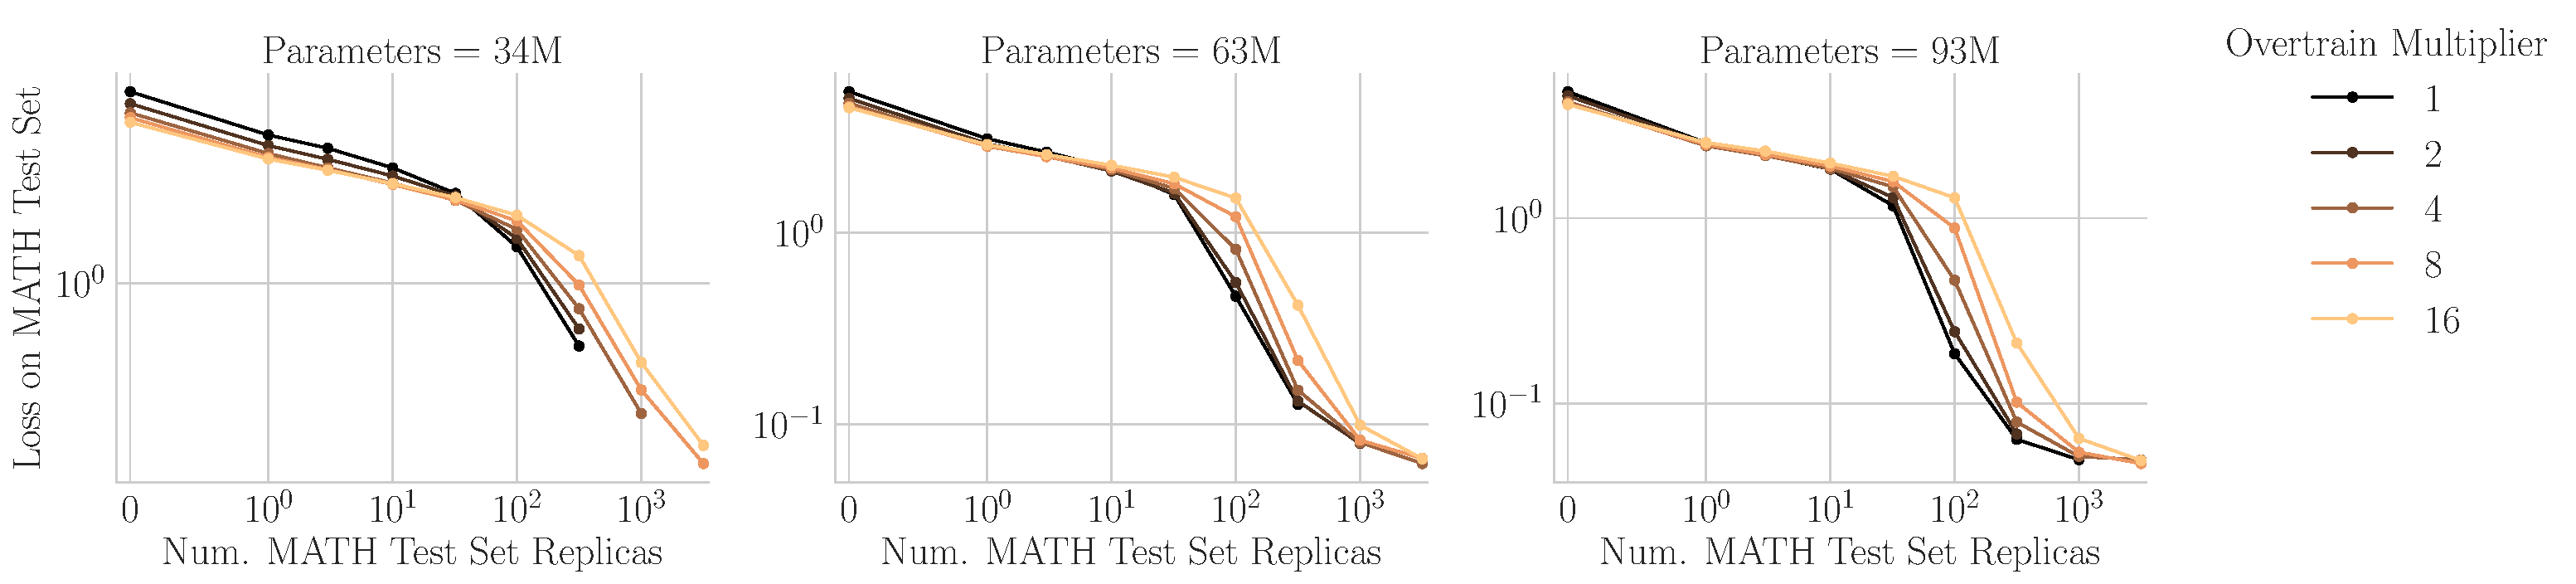
\includegraphics[width=\linewidth]{figures/10_math_qwen3_pt_cross_entropy/y=loss_x=num_replicas_hue=ot_col=params.pdf}
    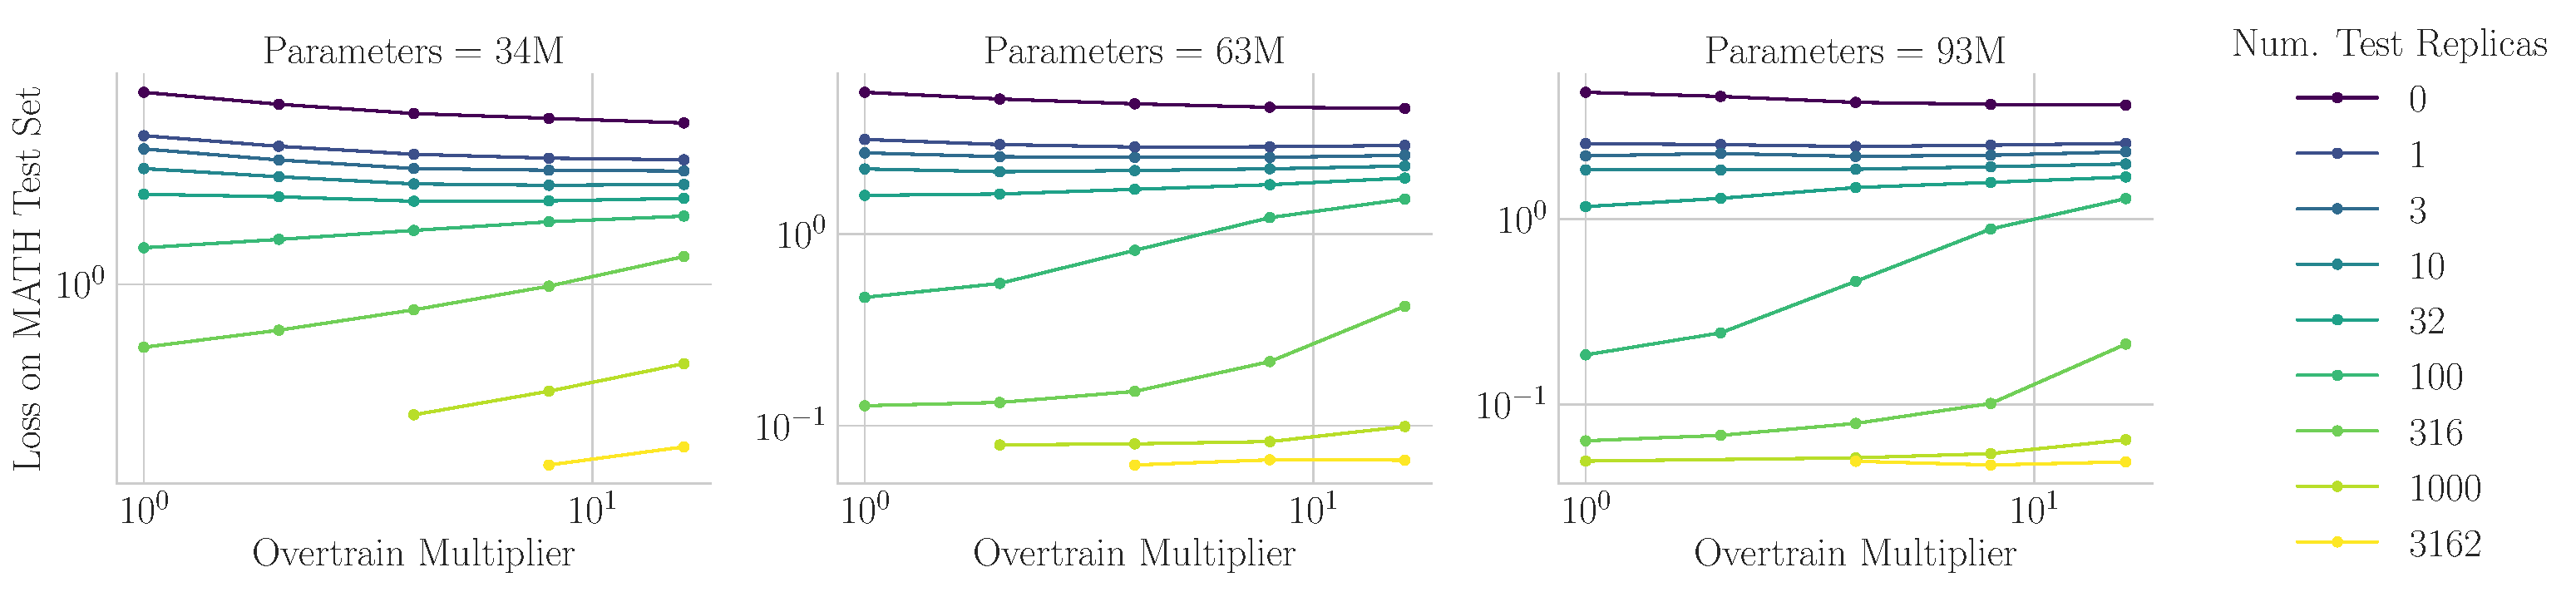
\includegraphics[width=\linewidth]{figures/10_math_qwen3_pt_cross_entropy/y=loss_x=ot_hue=num_replicas_col=params.pdf}
    \caption{\textbf{Overtraining with Fresh Data Mitigates Contamination.} Consistent with discriminative evaluations \citep{bordt2025howmuch}, overtraining (training longer than Chinchilla compute-optimal) on \emph{new fresh data} interacts with contamination: increasing overtraining decreases cross entropy on the MATH test set for uncontaminated models, but increases cross entropy for contaminated models. This suggests that while fresh data generally improves performance, it dilutes the ``dose,'' or proportion of contaminated pretraining tokens, thereby lessening the effect of the contamination. The crossover point shifts with model size, falling from 32 test set replicas for 34M to 1 replica for 93M models, indicating larger models lose their contamination advantage more readily when overtrained.}
    \label{fig:overtraining}
\end{figure*}
